\documentclass{scrartcl}
\usepackage{dominatrix}
\title{Optimizing DGEMM}
\subtitle{Group 16}
\date{Last Updated \today}
\author{Lim Mingjie, Kenneth (\href{mailto:kl545@cornell.edu}{kl545}) and Xinyi Wang (\href{mailto:xw327@cornell.edu}{xw327})}
\begin{document}
  \maketitle
  \section{Updates to Previous Work}
    This section describes modifications or alterations to the conclusions described in our previous submission.

    \subsection{Compiler Flags}

    We provide the compiler with the following flags to improve performance:
    \begin{verbatim}
  -fast -xHost -unroll-aggressive -ansi-alias
  -ftree-vectorize -restrict -parallel\end{verbatim}
    Loop vectorization attempts were characterized by inspecting the compiler's vectorization report, generated using the flags \verb|-qopt-report-phase=vec -qopt-report=5|. While the goal of this assignment was to optimize for performance on a single core, we also explored opportunities for automatic parallelization by making the GAP recommendations provided by the \verb|-guide| flag. In addition, we have also experimented with PGO by passing the flags \verb|-perf-gen/use -perf-dir|, but did not obtain any significant improvement from the baseline. This could have to do with the fact that we are running the binary on a slightly different architecture than that of the head node, and we have were not diligent in managing the profiler report that was generated.

    Compiler flags were tricky. On the side, we explored modifying the precision of the floating point operations (specifically, trying to decrease precision to see if it would give any improvement), using non-temporal writeback streams, and miscellaneous compiler annotations (\verb|#pragma simd|, etc.). Most of these attempts ended in failure.

    \subsection{Array Transpose}

    In the previous report, we found that explicitly transposing the array before performing any calculations improves the result because the stride length of the innermost loop is minimized. While this continues to be true, the optimizations introduced in the present work supercede the benefits obtained by transposing the array, turning it into a bottleneck instead. Therefore, we have opted to keep our the input indexed by column-major, and any transpose operations are performed \emph{when} we copy from the input to our working sets.

    \subsection{Blocking}

    Our previous attempts at blocking were a work in progress. We utilized a naive matrix multiplication kernel with some memory allocation optimizations largely based off the bootstrap code shipped with the assignment. Improving this has been the focus of our present efforts, and will be discussed in greater detail below.

    \subsection{Memory Alignment}

    In the previous report, we concluded that aligning data to a 16 byte boundary was ideal. After a review of the Intel Intrinsics documentation, we have revised this conclusion, and are now aligning data to a 32 byte boundary to maximize support for AVX instructions. In addition, we prepend relevant for-loops with the compiler annotation \verb|#pragma vector aligned| to enforce skipping of memory boundary checks within the loop.
  \section{Building a Fast Multiplication Kernel}
  Implicit in any blocked multiply implementation is the existence of a fast subroutine that is capable of multiplying two smaller matrices very rapidly. Our previous submission used a naive nested-loop approach, which was augmented significantly by good compiler optimizations.

  Our current approach makes heavy use of AVX instructions to provide a theoretical 4x speedup. We soon discover that emphasis needs to be placed on \emph{theoretical}, but we bravely proceed. Since the total length of the input to these instructions is 256 bits long, we can accomodate 4 double precision floating point numbers within one operation. However, this requires some modification to the cannonical matrix multiplication algorithm.

  Consider matrix $\mathbf{A}$ of size $4 \times P$ indexed by column-major, and matrix $\mathbf{B}$ of size $P \times 4$, also indexed by column-major. The result $\mathbf{C} = \mathbf{AB}$ is such that $\mathbf{C}$ has dimensions $4 \times 4$. The algorithm is as follows:
  \begin{enumerate}
    \item Simultaneously load all 4 elements in column $i$ of $\mathbf{A}$. Call this $\mathbf{A}_i$.
    \item Broadcast an element at index $k, j$ of $\mathbf{B}$ into all 4 positions of a \verb|ymm| register. Call this $\mathbf{B}_{kj}$.
    \item Simultaneously multiply $\mathbf{A}_i$ with $\mathbf{B}_{kj}$ element-wise. This is the equivalent of a dot-product for each element of $\mathbf{A}_i$ with $\mathbf{B}_{kj}$.
    \item Sum the result of (3) element-wise over all $i$. This yields the $k$-th column of $\mathbf{C}$.
  \end{enumerate}
  This approach is largely inspired by \verb|kdgemm.c| provided in the reference tuning repository. In homage, we refer to this algorithm henceforth as `$4P4$ multiplication'. \autoref{fig:avx-1} shows a preliminary benchmark of this approach.

  \begin{figure}[ht!]
    \centering
    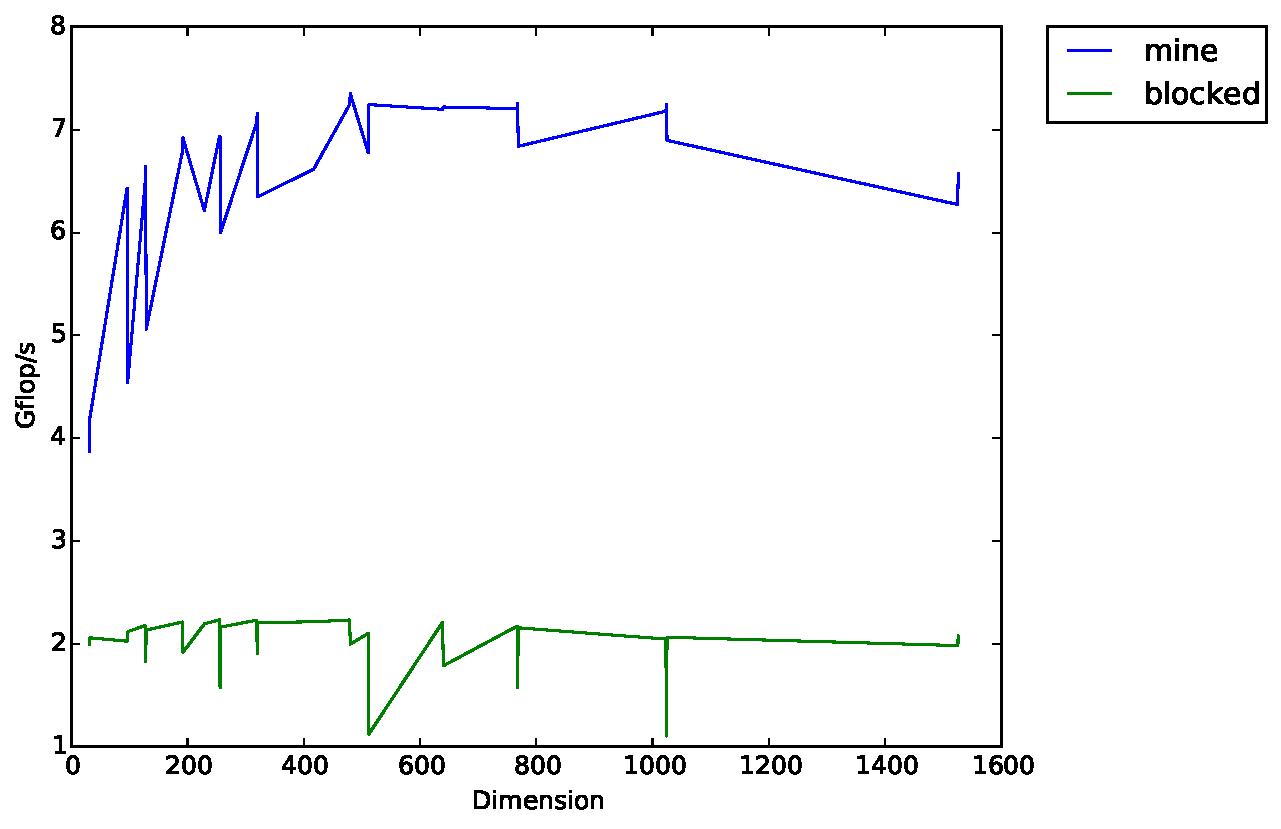
\includegraphics[width=\textwidth]{timing-avx-4}
    \caption{Comparison of a kernel using AVX instructions (`mine') vs non-AVX instructions (`blocked') for a standard block multiplication scheme using a block size of $4 \times 4$.\label{fig:avx-1}}
  \end{figure}

  Since we are loading from $\mathbf{A}$ in column order, there is no need to transpose $\mathbf{A}$ to row-major. This allows us to save on the preallocation needed for scratch memory, and more importantly, means that the kernel does not incur an $O(P^2)$ matrix transpose cost on every run. This is significant at large values of $P$. We note with interest that groups which attempted a transpose tended to have diminishing returns as the matrix dimensions increase, whereas our approach is relatively stable. We discuss the effects of memory allocation and copy optimization in greater detail in the eponymous section.

  A second advantage is a significant speedup due to the number of operations that must be performed. Naive matrix multiply uses the following instruction tally:
  \begin{itemize}
    \item $P$ load operations for a row in $A$
    \item $P$ load operations for a column in $B$
    \item $P$ multiply operations for a row-column dot-product
    \item $\log P$ additions for the partial sum
    \item $P$ write operations for a column in $C$
  \end{itemize}
  In contrast, the use of AVX instructions allows us to update all 4 columns on every loop (iterating over $P$) with just 12 instructions. The performance gains are somewhat debatable. It can be argued that a naive nested loop that is correctly annotated can benefit tremendously from automatic vectorization\footnote{Inspecting the decompiled assembly instructions for a naive matrix multiply reveals, indeed, that a non-trivial amount of AVX instructions are incorporated into the mix. ICC knows what it's doing!}, but we feel that being explicit with our intentions sets the stage for subsequent work, if any.

  \section{Copy Optimization}
  The second prerequisite for blocking is the efficient use of memory. The nature of row-column style matrix multiplication suggests that one benefits from keeping a row of $\mathbf{A}$ in memory and using that in the computation of all columns of $\mathbf{B}$. On function initialization, we preallocate `dirty' memory in accordance with the size of the blocks we expect to be working with, and continually reuse the same memory space for all our computations. There are no synchronization issues to be mindful of because we are working in a single-threaded environment. An additional advantage is that careful selection of the array indices allows us to transpose the matrix, or concatenate orderings across strides, purely as a byproduct of the copying process.

  \begin{figure}[ht!]
    \centering
    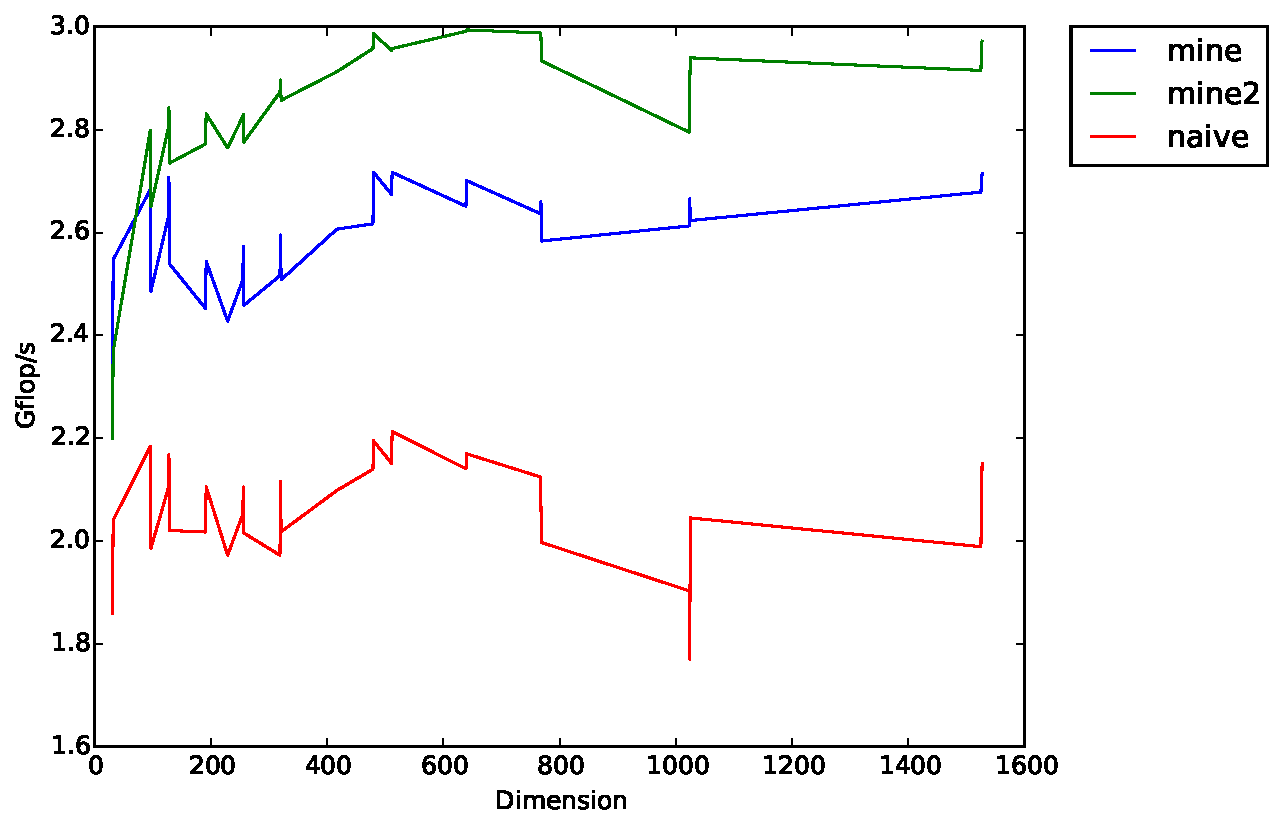
\includegraphics[width=\textwidth]{timing-malloc-comparison}
    \caption{Comparison of different copy optimization schemes using a representative example. `naive' follows mathematical intutition by transposing $\mathbf{A}$ to row-major prior to blocking, then transposing back to column-major within the kernel to ensure that memory access is contiguous. `mine' improves on `naive' slightly by preallocating scratch space for the transpose operation, and utilizing a tuned transpose function with fully unrolled loops (for a $4 \times 4$ matrix). `mine2' eliminates explicit transpose operations entirely.\label{fig:avx-2}}
  \end{figure}

  In the design of the kernel described in the foregoing section, we experimented with inputs indexed either by row-major or column-major. While we ultimately receive both inputs in column-major, see that one cannot extract a contiguous block from the input and pass it directly to the kernel\footnote{Both matrices are in column-major, but their dimensions are different. As such, some form of concatenation is required}. Copying \emph{creates} a contiguous block that is optimized for matrix multiplication, and we are at liberty to write the result---also contiguous in memory---back to the accumulating array when the operation is completed.

  \section{Striping The Inputs}
  Our attempts at crafting a good blocking solution using the foregoing kernel were deeply unsatisfying. We started by building the $4P4$ multiplication up to a $64 \times 64$ multiplication\footnote{The value $64$ is chosen here because we consider that the working memory for $\mathbf{A}$, $\mathbf{B}$ and $\mathbf{C}$ have to fit within the L2 cache, which is of size 256Kb. The next power of 2 is 128, which will overflow the cache size.}. Inputs were partitioned into blocks of size $64 \times 64$, zero-padding in cases where there were insufficient elements to fill the block completely. An unfortunate consequence of wrangling data into a format that fits the $64 \times 64$ schema is a small amount of overhead associated with extracting the block from the parent matrix. We minimize the time cost here by applying AVX instructions once again, to copy in vectors of 4 numbers. Note that this does not cause problems when copying odd-sized arrays because we have already zero-padded the input.

  The dominant problem with the blocked approach is that while it is capable of achieving a high maximum flop rate (approx. 12GFlops), it's performance fluctuates when crossing over an input whose size is a multiple of the block size. For example, an input with size $65 \times 65$ inevitably results in a computation for a $128 \times 128$ matrix, because the outlying element in both dimensions is zero-padded to form another $64 \times 64$ block. Nasty. This problem could be solved by applying an adaptive approach that varies the block size across the parent matrix --- `large' blocks of 64 at the start, and the smallest usable power of 2 close to the edges. We explored the idea briefly, but the complexity of such a solution prevented us from going further within this window of execution.

  \begin{figure}[ht!]
    \centering
    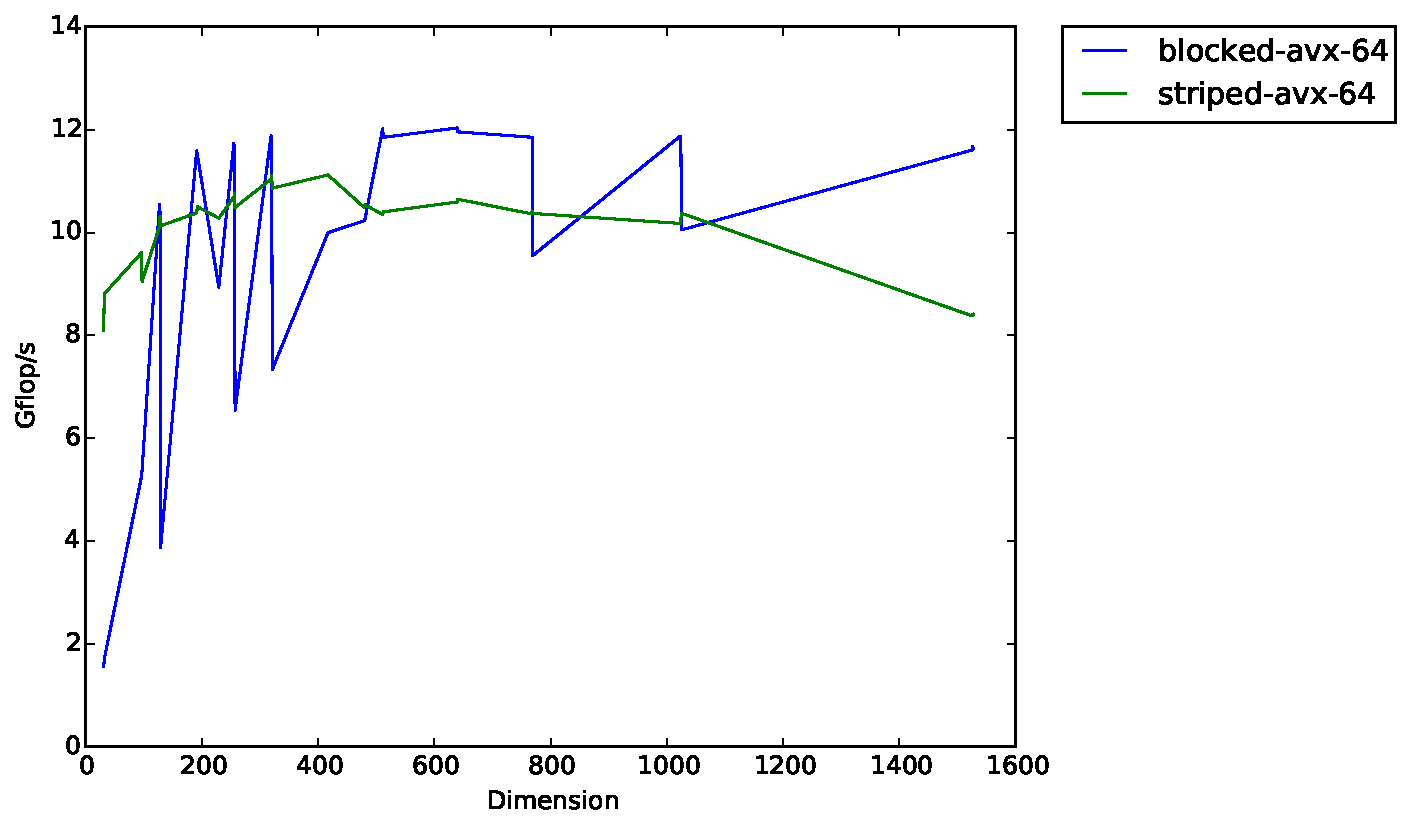
\includegraphics[width=\textwidth]{timing-blocked-vs-striped}
    \caption{Comparison of a blocked matrix multiply scheme (`blocked-avx-64') vs. a striped matrix multiply scheme (`striped-avx-64').\label{fig:avx-2}}
  \end{figure}

  Instead, we considered using a striped approach that exploits the $4P4$ nature of the kernel. That is, we ``stripe'' the input in rows or columns of 4, leaving the other dimension unmodified.  The immediate advantage of doing so is a decrease in the amount of diligence required to handle the copying (and thence, a small performance boost here and there). Once $\mathbf{A}$ is converted to row-major, it is a simple matter of extracting contiguous blocks of memory and multiplying them by equally contiguous blocks of memory from $\mathbf{B}$. We compare the results of both a blocked approach and striped approach in \autoref{fig:avx-2}.

  See that while the striped approach does not ultimately achieve the same maximum performance as the blocked approach, it is a lot more consistent over the range of input. For this reason, we cite the striped matrix multiply scheme as our preferred method.

  The striped approach is not without flaws. The performance drops as the dimensions increase because each stripe that is passed to the kernel is successively larger, whereas the blocked approach clamps the kernel size to $64 \times 64$ regardless of the input size. One can conceive of a hybrid approach in which we block only when it is appropriate to do so (e.g.~the dimensions of the input are close to multiples of 64), and fall back to the striped approach otherwise.
  \section{Conclusion}
  \begin{figure}[ht!]
    \centering

    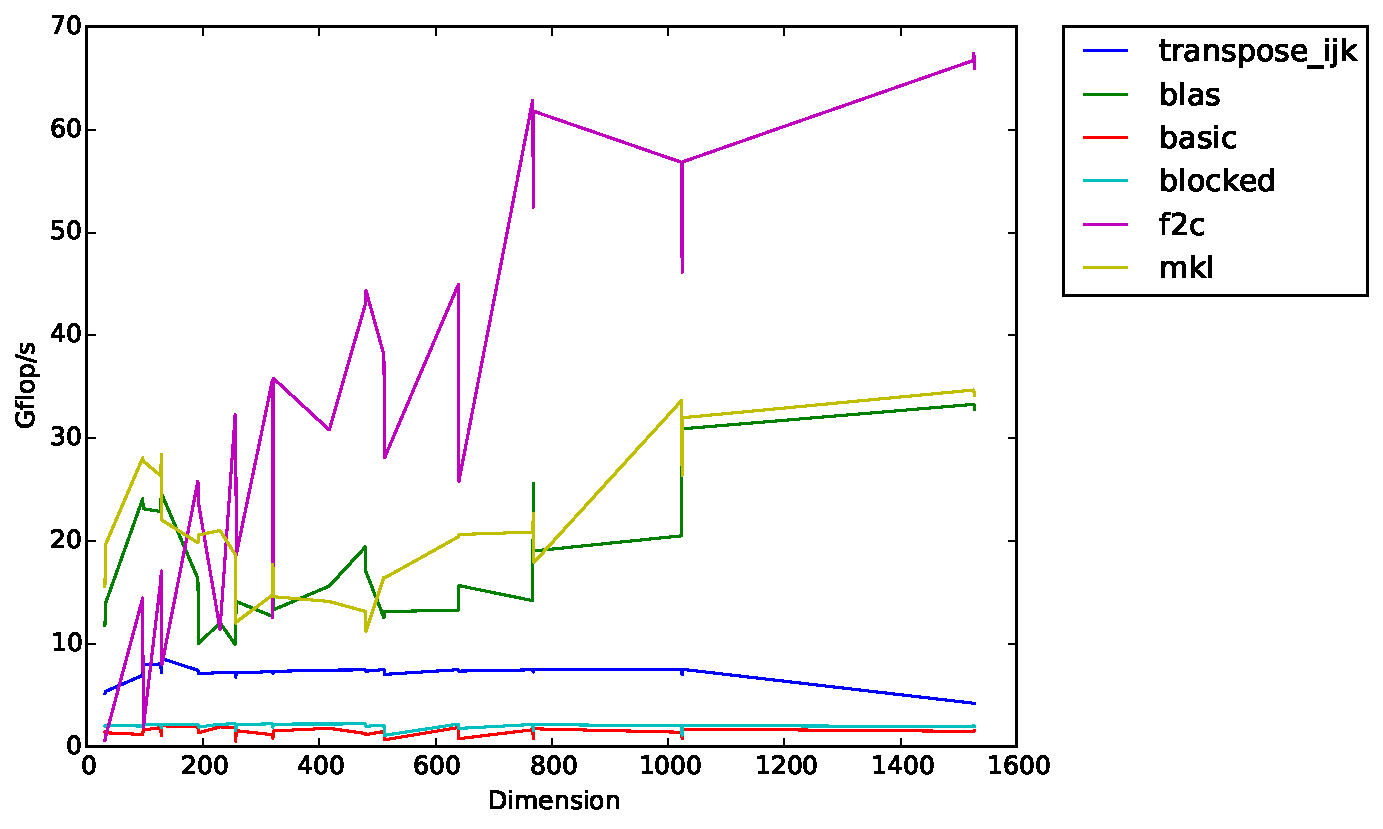
\includegraphics[width=\textwidth]{timing-current-best}
    \caption{Previous best results.\label{fig:avx-prev}}

    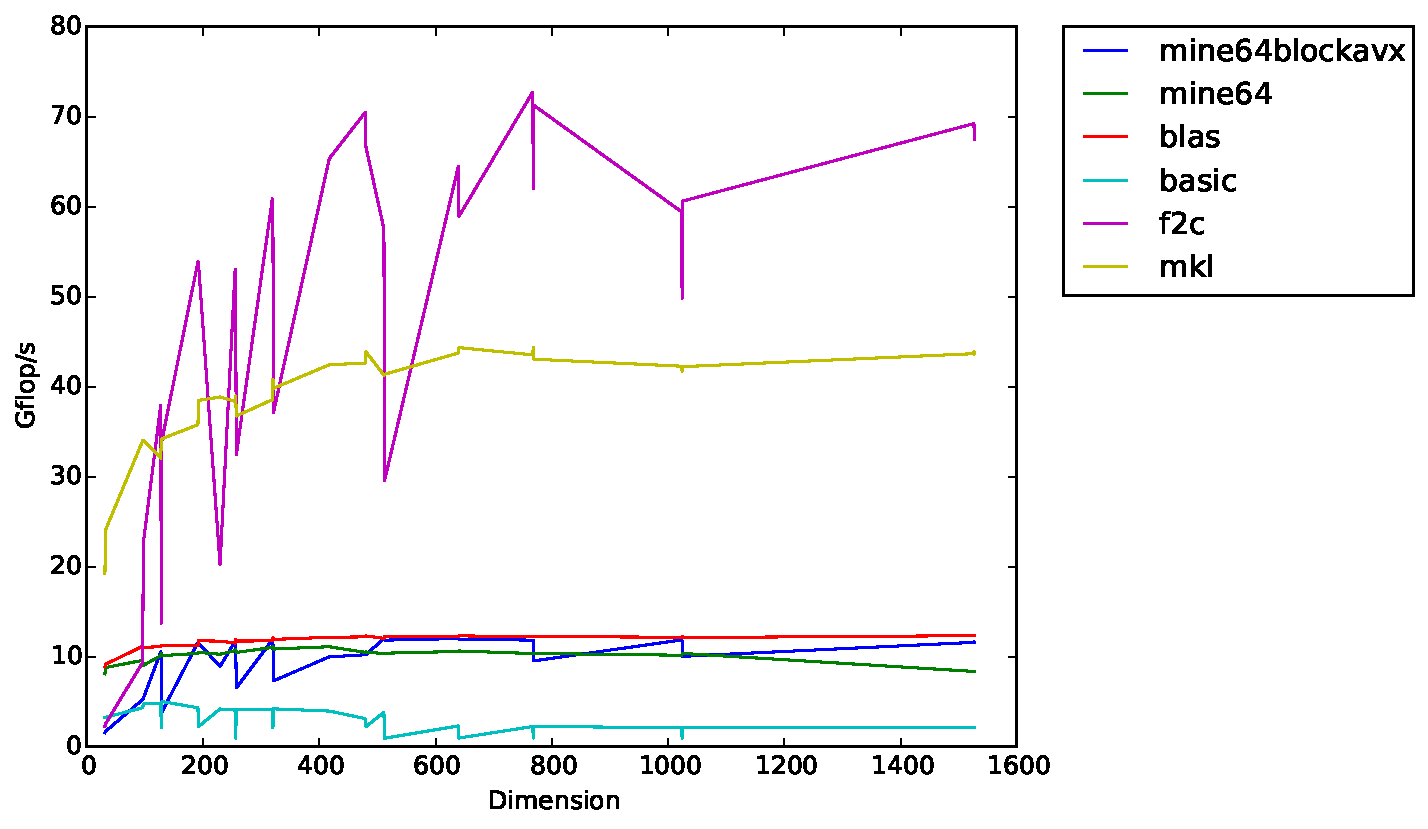
\includegraphics[width=\textwidth]{timing-final-best}
    \caption{Current best results.\label{fig:avx-final}}
  \end{figure}
  We have made a modest improvement over our previous results. For comparison, \autoref{fig:avx-prev} shows our previous best result, whereas \autoref{fig:avx-final} shows our current best results. We note with interest that while many other groups report better-than-blas performance, BLAS appears to perform at around a 10GFlops benchmark for them. We were careful to apply the same compiler flags to all components of the benchmark, resulting in an approx. 30GFlops benchmark for us. It is ultimately still difficult to beat purpose-built and well-tuned linear algebra libraries. Let's not even talk about Fortran...
\end{document}
